
\chapter{Разработка программы решения теоретико-графовой задачи на
  языке программирования C++}

В следующем разделе я описываю выполнение второго этапа расчетной
работы на примере задачи поиска одного из минимальных путей в
неориентированном графе. Для понимания руководства студент должен
обладать следующими знаниями:

\begin{itemize}
\item базовыми знаниями по языку C++;
\item базовыми знаниями по работе с STL-контейнерами std::set,
  std::map, std::list, std::pair.
\end{itemize}

\section{Задание}

На этом этапе выполнения расчетной работы вам необходимо будет
разработать программу с использованием библиотеки моделирования
sc-памяти, которая бы решала вашу теоретико-графовую задачу на основе
формализации предметной области, проведенной на предыдущем этапе. Сам
алгоритм вы уже исследовали в прошлом семестре, но сейчас надо будет
не просто реализовать какой-то алгоритма, а адаптировать его к
графодинамическому способу обработки информации. Это значит, что вся
информация, необходимая для работы вашего алгоритма, должна храниться
в sc-памяти и там же и обрабатываться. В качестве примера
<<неудобства>>, которое вам может принести такое требование, я могу
привести невозможность использования привычной матрицы
смежности/инцидентности.  Поэтому для прохождения этого этапа вам
придется взглянуть на алгоритм, решающий выбранную задачу, под другим
углом.

В качестве тестов для написанной программы необходимо использовать
тестовые примеры, которые вы сделали в ходе предыдущего этапа
расчетной работы.

\section{Установка и настройка рабочей среды}

Для начала мы установим и настроим рабочую среду для программирования
с использованием программной модели sc-памяти и запустим
программу-пример, которая использует эту модель. Всё описанное в этой
главе программное обеспечение можно найти как в интернете, так и на
кафедральном сервере info. На сервере info весь материал и всё
программное обеспечение располагается по следующему пути:
\begin{verbatim}
\\Info\StudInfo\~Методическое обеспечение кафедры\~Учебные курсы\2 курс\ППвИС\@Расчётная работа
\end{verbatim}

Во-первых, нам необходимо скачать и установить программный модуль
sc-core, который представляет собой ядро для обработки
sc-текстов. Инсталлятор для этого модуля можно взять в следующих
местах:

\begin{itemize}
\item скачать из папки
  \href{http://sourceforge.net/projects/ostis/files/kpm/}{kpm}
  sc-core-0.2.5-win32.exe (работает с MS Visual Studio 9)
\item скачать по следующему пути sc-core-0.2.5.exe (работает с MS
  Visual Studio 9):
\begin{verbatim}
\\Info\StudInfo\~Методическое обеспечение кафедры\~Учебные курсы\2 курс\ППвИС\@Расчётная работа\sc-core-0.2.5.exe
\end{verbatim}
\item скачать по следующему пути sc-core-0.2.5-vc10-bin-win32.exe
  (работает с MS Visual Studio 10):
\begin{verbatim}
\\Info\StudInfo\~Методическое обеспечение кафедры\~Учебные курсы\2 курс\ППвИС\@Расчётная работа\sc-core-0.2.5-vc10-bin-win32.exe
\end{verbatim}
\end{itemize}

После того, как вы скачали инсталлятор, запустите его. Желательно
устанавливать sc-core так, чтобы полный путь к установленной папке не
содержал пробелов в именах директорий. При установке необходимо
выбрать опцию, которая добавит директорию исполняемых файлов sc-core в
переменную среды окружения \verb+PATH+ (см. рис.~\ref{fig:Add_sc_core_to_path}).

\begin{figure}[h]
  \centering
  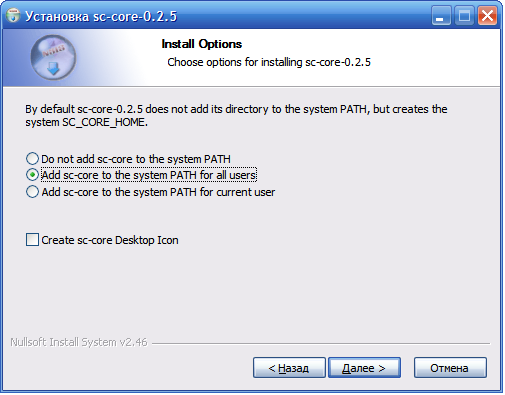
\includegraphics[scale=0.7]{images/4/setup/Add_sc_core_to_path}
  \caption{Добавление директории исполняемых файлов sc-core в
    системную переменную PATH для всех пользователей}
  \label{fig:Add_sc_core_to_path}
\end{figure}
 
Мной была выбрана установка sc-core в папку
\verb+"c:\\sc-core"+. После установки данного модуля были изменены
следующие переменные среды окружения:
\begin{itemize}
\item \verb+SC_CORE_HOME+, которая теперь имеет значение
  \verb+"c:\sc-core"+
\item \verb+PATH+, к которой была добавлена директория
  \verb+"c:\sc-core\bin"+
\end{itemize}

В дальнейшем для указания пути к директории sc-core я буду
использовать значение переменной среды окружения \verb+SC_CORE_HOME+.

Для сборки примера нам еще будет необходима программа
CMake. Необходимо скачать установочный файл для версии не ниже 2.6.2
или взять инсталлятор из папки расчетной работы на сервере info. Как и
при установке sc-core, при установке CMake необходимо выбрать опцию,
которая добавит директорию исполняемых файлов в переменную среды
окружения \verb+PATH+ (см. рис.~\ref{Add_cmake_to_path}).
 
\begin{figure}[h]
  \centering
  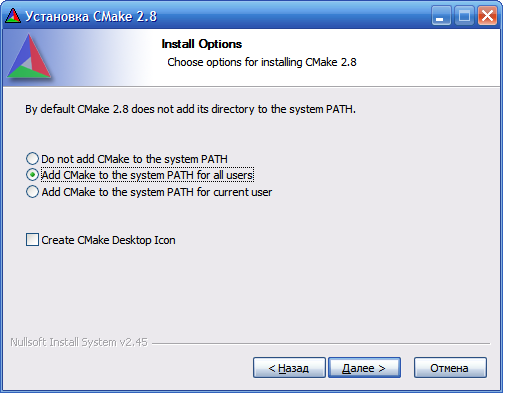
\includegraphics[scale=0.7]{images/4/setup/Add_cmake_to_path}
  \caption{Добавление CMake в системную переменную PATH для всех
    пользователей}
  \label{fig:Add_cmake_to_path}
\end{figure}

С модулем sc-core версии 0.2.5 идет старая версия примера
использования библиотеки моделирования sc-памяти, поэтому я рекомендую
вам взять из папки на сервере info файл с именем
\verb+wave_find_path.cpp+ и скопировать его в приеденную ниже папку,
заменив существующий там файл с таким именем. После этого перейдем к
генерации проекта для примера:
\begin{verbatim}
%SC_CORE_HOME%\examples\wave_find_path
\end{verbatim}

Для генерации проекта примера воспользуемся консолью. Для запуска
консоли нажимаем клавиши \verb|Win + R|, в появившемся диалоге пишем cmd и
нажимаем Enter. На экране должно появиться следующее окно, как
показано на рисунке 2.3.

\begin{figure}[h]
  \centering
  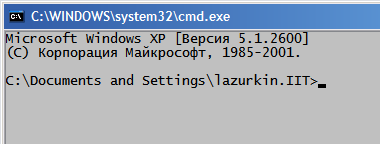
\includegraphics[scale=0.7]{images/4/setup/Run_console}
  \caption{Открытая консоль}
  \label{fig:Run_console}
\end{figure}

Переходим в директорию примера использования библиотеки моделирования
sc-памяти, используя команды:
\begin{verbatim}
c: 
cd %SC_CORE_HOME%\examples\wave_find_path
\end{verbatim}

%\begin{figure}[h]
%  \centering
%  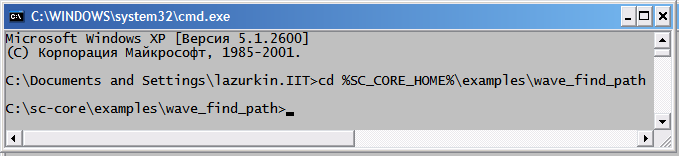
\includegraphics[scale=0.7]{images/4/setup/Cd_to_example_dir}
 % \caption{Переход в директорию примера wave\_find\_path}
  %\label{fig:Cd_to_example_dir}
%\end{figure}

% Если у вас Windows с русификацией, то могут возникнуть проблемы с запуском cmake. CMake будет сообщать о том, что он не может скопировать файлы "CMakeVSMacros1.vsmacros" и "CMakeVSMacros2.vsmacros" в "c:\Documents and Settings\lazurkin.IIT\Мои документы\Visual Studio 2008\Projects\VSMacros80\CMakeMacros" (это путь на моей файловой системе с моим именем пользователя, для вас он будет отличаться названием директории вашего пользователя). Эти файлы необходимо скопировать вручную. Для этого просто скопируйте содержимое "c:\Program Files\cmake2.8\share\cmake-2.8\Templates\" в "c:\Documents and Settings\lazurkin.IIT\Мои документы\Visual Studio 2008\Projects\VSMacros80\CMakeMacros" (этот путь для вас будет другой!!!). 

% При помощи следующей команды сгенерируем проект MS Visual Studio 9.0
% для сборки и запуска примера (в cmake есть генератор и для MS Visual
% Studio 10.0, просто введите команду cmake и на консоль будет выведен
% список всех доступных генераторов):

% cmake -G "Visual Studio 9 2008" .

 
% Рисунок 2.5 Генерация проекта для примера wave_find_path 
% Если у вас MS Visual Studio 2010, то можете попробовать команду:
% cmake .

% После корректной работы CMake в директории будет создан проект wave_find_path. Открываем его при помощи MS Visual Studio 9.0. Нажимаем правой кнопкой мыши на проекте wave_find_path в Solution Explorer и выбираем пункт меню "Set as StartUp Project". После этого название данного проекта будет выделено жирным цветом. Теперь можно запустить на исполнение пример wave_find_path (пример вывода на рисунке 2.6).
 
% Рисунок 2.6 Вывод работы программы-примера wave_find_path

\section{Назначение и структура модуля sc-core}

Модуль sc-core – это набор библиотек и программ, которые составляют
ядро обработки sc-текстов. В него входят следующие динамические
библиотеки:
\begin{itemize}
\item libsys : библиотека, обеспечивающая независимость от
  операционной системы;
\item libtgf : библиотека обработки формата TGF (Transfer Graph Format);
\item libsc : библиотека моделирования sc-памяти;
\item libpm : библиотека процессорного модуля для обработки sc-текстов
  (например, она включает scp-интерпретатор и навигационно-поисковую
  машину);
\item librgp : библиотека удаленного подключения к sc-памяти по
  протоколу RGP (Remote Graph Protocol).
\end{itemize}

Также модуль sc-core включает следующие программы:
\begin{itemize}
\item start-pm : средство запуска процессорного модуля из консоли;
\item dumptgf : утилита для просмотра TGF-файлов в человеко-читаемой
  форме;
\item scs2tgf : транслятор sc.s-текстов в формат TGF.
\end{itemize}

Как вы уже знаете, при установке инсталлятор модуля sc-core создает
переменную среды \verb+SC_CORE_HOME+, которая в качестве своего значения
будет иметь путь к корневой папке установленного модуля. Если вы
заглянете в эту папку, то сможете увидеть следующую структуру папок и
файлов (пути даются относительно значения переменной окружения
\verb+SC_CORE_HOME+):
\begin{itemize}
\item \verb|bin/| : бинарные файлы библиотек и программ. В этой директории
  динамические библиотеки для отладочной версии приложения имеют в
  конце имени букву «d» (сравните, libSCd.dll и libSC.dll);
\item \verb|doc/| : doxygen-документация на английском языке по модулю sc-core;
\item \verb|examples/| : примеры использования модуля:
  \begin{itemize}
  \item \verb|wave_find_path/| : С++-пример использования библиотеки
    sc-памяти libsc на основе алгоритма поиска одного из минимальных
    путей в неориентированном графе;
  \item \verb|fs_repo_src/| : SCP-пример на основе алгоритма поиска одного из
    минимальных путей в неориентированном графе;
  \end{itemize}
\item \verb|include/| : содержит директории с заголовочными файлами для всех библиотек
  модуля;
\item \verb|lib/| : библиотеки импорта для всех динамических библиотек модуля
  В этой директории библиотеки импорта для отладочной версии
  динамической библиотеки имеют в конце имени букву «d» (сравните,
  libSCd.lib и libSC.lib);
\item \verb|share/| : содержит дополнительные необходимые ресурсы для работы
  модуля, которые нельзя отнести ни в одну из уже описанных
  директорий.
\end{itemize}

Из всего описанного выше в контексте данного руководства нас будет
интересовать библиотека моделирования sc-памяти libsc и пример ее
использования \verb|wave_find_path|. В ходе дальнейшего разговора мы сначала
будем рассматривать основные понятия, структуру и классы библиотеки
libsc, а затем перейдем к более конкретному рассмотрению примера
использования этой библиотеки.

\section{Библиотека моделирования sc-памяти – libsc}

В данном разделе мы рассмотрим библиотеку моделирования sc-памяти в
объеме, необходимом для выполнения это этапа расчетной работы.

\subsection{Общие сведения}

Библиотека моделирования sc-памяти написана на языке C++, поэтому в
этом разделе мы будем рассматривать в основном классы для
моделирования sc-памяти и их методы, а также некоторые функции попадут
в поле нашего зрения. Однако сейчас давайте рассмотрим файлы и
директории из модуля sc-core, которые имеют отношение к библиотеке. И
так, приступим (пути даются относительно значения переменной окружения
\verb|SC_CORE_HOME|):
\begin{itemize}
\item \verb|bin/libSCd.dll| : debug-версия динамической библиотеки
  моделирования sc-памяти;
\item \verb|bin/libSC.dll| : release-версия динамической библиотеки
  моделирования sc-памяти;
\item \verb|lib/libSCd.lib| : библиотека импорта для динамической библиотеки
  libSCd.dll;
\item \verb|lib/libSC.lib| : библиотека импорта для динамической библиотеки
  libSC.dll;
\item \verb|doc/sc-core/| : общая doxygen-документация по модулю
  sc-core, в том числе и по рассматриваемой библиотеке libsc;
\item \verb|include/libSC/| : заголовочные файлы рассматриваемой
  библиотеки;
\item \verb|examples/wave_find_path| : пример использования
  рассматриваемой библиотеки.
\end{itemize}

Библиотека libsc зависит от библиотеки обработки формата TGF libtgf, к
которой относятся следующие директории и папки (пути даются
относительно значения переменной окружения \verb|SC_CORE_HOME|):

\begin{itemize}
\item \verb|bin/libTGFd.dll| : debug-версия динамической библиотеки
  libtgf (она необходима для работы с libSCd.dll);
\item \verb|bin/libTGF.dll| : release-версия динамической библиотеки
  libtgf (она необходима для работы с libSC.dll);
\item \verb|include/libTGF/| : заголовочные файлы библиотеки libtgf;
\end{itemize}

Теперь перейдем к непосредственному описанию библиотеки libsc.

\subsection{Сегментная модель sc-памяти}

Когда вы занимались формализацией на SCg по курсу МОИС, то считали,
что sc-элементы с одинаковыми идентификаторами должны
склеиться. Однако в реализации sc-памяти используется сегментная
модель и поэтому всё несколько сложнее.

В сегментной модели вся память разбивается на sc-сегменты, где каждый
sc-элемент принадлежит ровно одному сегменту. Уникальность
идентификаторов sc-элементов имеет место только в рамках
sc-сегмента. Сами sc-сегменты могут организовываться в рамках
sc-директории. Проиллюстрирую на конкретной структуре sc-памяти:

\begin{itemize}
\item /: корневая sc-директория, которая всегда существует
  
  \begin{itemize}
  \item \verb|graph_theory/|: sc-директория, которая содержит базу знаний по
    теории графов
    \begin{itemize}
    \item \verb|keynode|: sc-сегмент, который содержит ключевые
      узлы базы знаний по теории графов
      \begin{itemize}
      \item \idtf{графовая структура}
      \item \idtf{вершина\_}
      \item \idtf{связка\_}
      \item \idtf{неориентированный граф}
      \item \idtf{ребро\_} и т.д.
      \end{itemize}
    \end{itemize}

  \item \verb|tmp/|: содержит sc-сегменты для временной обработки
    sc-конструкций
    \begin{itemize}
    \item \verb|wave_find_path| : временный sc-сегмент для работы алгоритма
      поиска одного из минимальных путей в неориентированном графе
    \end{itemize}

  \item \verb|proc/|: содержит системные sc-сегменты;
    \begin{itemize}
    \item \verb|keynode|: sc-сегмент, который содержит системные ключевые
      узлы
      \begin{itemize}
      \item \idtf{1\_}
      \item \idtf{2\_} и т.д.
      \end{itemize}
    \end{itemize}
  \end{itemize}
\end{itemize}

Такая структура sc-директорий и sc-сегментов аналогична структуре
папок и файлов на файловой системе. Аналогом файла является
sc-сегмент, а аналогом содержимого файла является sc-конструкции. В
сегментной модели любой объект (sc-директория, sc-сегмент, sc-элемент)
может быть однозначно идентифицирован при помощи строки особого вида,
которая по историческим причинам называется URI (Universal Resource
Identifier). Формат URI аналогичен формату пути к папке или файлу на
файловых системах Unix-подобных операционных систем. Вот некоторые
примеры URI:

\begin{itemize}
\item \verb|/|: URI sc-директории
\item \verb|/graph_theory/keynode| : URI sc-сегмента
\item \verb|/graph_theory/keynode/вершина_| : URI sc-элемента
\end{itemize}

Адресация sc-элементов с использованием URI удобна для человека, но
неудобна для компьютера, поэтому существует понятие
sc-адреса. SC-адрес – это некоторое число, которое однозначно
идентифицирует sc-элемент в сегментной модели sc-памяти. С
использованием sc-адресов sc-элементов ведется их обработка в рамках
sc-сессии. SC-сессия - это логически единая последовательность
операций над некоторой областью sc-памяти (sc-директориями,
sc-сегментами, sc-элементами). Для того, чтобы получить доступ к
данным sc-сегмента, нужный sc-сегмент должен быть открыт в рамках
используемой sc-сессии. Существует особый вид sc-сессии, который
называется системная sc-сессия, в рамках которой все существующие
sc-сегменты всегда открыты.

Я думаю, что читатель уже получил общие сведения о том, что такое
сегментная модель, sc-директория, sc-сегмент, URI, sc-адрес,
sc-сессия, поэтому в следующем разделе я начну рассматривать
практические вопросы использования библиотеки моделирования sc-памяти.

\subsection{Начало работы с библиотекой libsc}

В прошлом разделе мы рассмотрели логическое устройство сегментной
модели sc-памяти, а теперь проведем аналогию с текущей реализацией на
языке программирования С++.

Понятию sc-сегмента в библиотеке libsc соответствует класс
\lstinline{sc_segment}, который описан в файле
\verb|sc_segment.h|. Понятию sc-адреса соответствует
\lstinline{typedef sc_addr} из заголовочного файла \verb|sc_types.h|,
а sc-сессии – класс \lstinline{sc_session} из \verb|libsc.h|. Для
представления URI и идентификаторов sc-элементов используется
\lstinline{typedef sc_string} (это просто другое имя для
\lstinline{std::string}), объявленный в \verb|sc_types.h|. Чтобы
начать работу со всеми этими типами, достаточно подключить только один
заголовочный файл, а именно \verb|libsc.h|, потому что в него включены
и \verb|sc_segment.h|, и \verb|sc_types.h|.

Работа с объектами классов \lstinline{sc_session} и
\lstinline{sc_segment} всегда ведется через указатель на объект,
поэтому методы и функции, которые возвращают указатель на объекты этих
классов, могут возвращать \lstinline{0} или \lstinline{NULL}, чтобы
показать наличие ошибки в процессе выполнения. Если в тексте ниже я
буду писать о работе с объектами классов \lstinline{sc_session} и
\lstinline{sc_segment}, то это почти всегда надо понимать, как работу
с такими объектами через указатель.

Рассмотрим, как обстоят дела в этом плане с типом
\lstinline{sc_addr}. В \verb|sc_types.h| он объявлен следующим образом:
\begin{lstlisting}
  typedef sc_global_addr *sc_addr;
\end{lstlisting}

Как видно из приведенного выше объявления, \lstinline{sc_addr} – это
указатель на класс \lstinline{sc_global_addr}. Поэтому методы и
функции, которые возвращают \lstinline{sc_addr}, могут возвращать
\lstinline{0}, \lstinline{NULL} или \lstinline{SCADDR_NIL} (это
\lstinline{define} для \lstinline{0}), чтобы показать наличие ошибки в
процессе выполнения. В отличие от \lstinline{sc_session} и
\lstinline{sc_segment}, с типом \lstinline{sc_addr} мы работаем без
указателя, потому что \lstinline{sc_addr} – это и так указатель
(просто другое имя для указателя на
\lstinline{sc_global_addr}). Напоследок об \lstinline{sc_addr} стоит
сказать следующее:
\begin{itemize}
\item для переменных этого типа можно использовать операторы
  \lstinline{==} и \lstinline{!=}, чтобы проверить идет работа с одним
  и тем же sc-элементом или с разными;
\item у \lstinline{sc_global_addr} есть открытое поле
  \lstinline{sc_global_addr::seg}, которое позволяет получить
  sc-cегмент, в котором находится адресуемый sc-элемент;
\item если в дальнейшем будет идти речь о работе с sc-элементами, то
  это значит, что речь идет о работе с соответствующими им
  sc-адресами.
\end{itemize}

Предыдущий текст должен был вас уже утомить, поэтому разбавим этот
раздел примерами кода. Для начала работы с моделью sc-памяти ее надо
инициализировать, это можно сделать вот так:

\begin{lstlisting}[texcl]
  #include <libsc.h>

  // $\dots$
  // Инициализируем sc-память при помощи функции \verb|libsc_init|.
  // Она вернет системную sc-сессию.
  // 
  sc_session *system = libsc_init();
\end{lstlisting}

Теперь необходимо инициализировать системные ключевые узлы (например,
\idtf{1\_}, \idtf{2\_} и др.). Все системные ключевые узлы объявлены в
заголовочном файле \verb|pm_keynodes.h| и инициализируются функцией
\lstinline{pm_keynodes_init}:

\begin{lstlisting}[texcl]
  #include <pm_keynodes.h>

  // $\dots$
  // Ключевые узлы будут созданы в sc-сегменте "/proc/keynode".
  // Например:
  //  - для работы с ключевым узлом \idtf{1\_} можно использовать имя \verb|N1_|
  //  - для работы с ключевым узлом \idtf{2\_} можно использовать имя \verb|N2_|
  //  - закономерность очевидна $\dots$
  //
  pm_keynodes_init(system);
\end{lstlisting}

В принципе уже можно работать с sc-памятью через системную sc-сессию
\lstinline{system}, но в идеале лучше работать через пользовательскую
sc-сессию:

\begin{lstlisting}[texcl]
  // Получим пользовательскую sc-сессию при помощи функции \verb|libsc_login|.
  //
  sc_session *session = libsc_login();

  // При помощи метода \verb|sc_session::open_segment| по URI "/proc/keynode"
  // откроем в нашей пользовательской sc-сессии sc-сегмент системных 
  // ключевых узлов.
  //
  session->open_segment(“/proc/keynode”);
\end{lstlisting}

Теперь создадим уникальный sc-сегмент для исследования работы
sc-памяти:

\begin{lstlisting}[texcl]
  // Этот заголовочный файл содержит функции, которые облегчают работу с 
  // sc-сегментами.
  #include <segment_utils.h>
  
  // $\dots$
  // Создадим уникальный sc-сегмент с использованием \verb|create_unique_segment|
  // и URI этого sc-сегмента будет начинатся с "/tmp/test".
  // 
  sc_segment *segment = create_unique_segment(session, “/tmp/test”);

  // Созданный при помощи sc-сессии session sc-сегмент будет автоматический
  // открыт в ней.
  //
\end{lstlisting}

Пользовательская sc-сессия \lstinline{session} и созданный sc-сегмент
\lstinline{segment} будут использоваться во всех дальнейших примерах
без какого-то явного объявления.

После окончания необходимой работы sc-память нужно почистить:
\begin{lstlisting}[texcl]
  // Удалим созданный sc-сегмент seg при помощи метода \verb|sc_session::unlink|
  // Метод \verb|sc_segment::get_full_uri| возвращает URI sc-сегмента.
  //
  session->unlink(segment->get_full_uri());

  // Закроем пользовательскую sc-сессию.
  //
  session->close();

  // Деинициализируем sc-память.
  //
  libsc_deinit();

  // Обратите внимани на то, что явно при помощи оператора \verb|delete| никакая 
  // память не освобождается. При работе с типами \verb|sc_session|, \verb|sc_segment|,
  // \verb|sc_addr| память явно освобождать не надо.
  //
\end{lstlisting}

Перед тем, как мы будем рассматривать операции генерации и поиска в
sc-памяти, вам еще нужно познакомиться со способом задания типа
sc-элементов, поэтому переходим к следующему разделу.

\subsection{Тип sc-элемента}

Для задания типа sc-элемента в библиотеке libsc используется С++-тип
\lstinline{sc_type}, который объявлен в файле
\verb|sc_types.h|. Значение типа \lstinline{sc_type} – это просто
число, которое является результатом операции побитового ИЛИ некоторых
числовых констант. Каждая из числовых констант задает значение
свойства из заранее определенного диапазона. Для выполнения расчетной
работы вам достаточно знать о следующих свойствах:

\begin{itemize}
\item Структурный тип sc-элемента. Используемые числовые константы
  С++:
  \begin{itemize}
  \item \lstinline{SC_UNDF}: sc-элемент неопределенного типа;
  \item \lstinline{SC_ARC}: sc-дуга;
  \item \lstinline{SC_NODE}: sc-узел.
  \end{itemize}

\item Константность sc-элемента. Используемые числовые константы С++:
  \begin{itemize}
  \item \lstinline{SC_CONST}: константность;
  \item \lstinline{SC_VAR}: переменность;
  \item \lstinline{SC_METAVAR}: метапеременность.
  \end{itemize}

\item Нечеткость sc-дуги. Используемые числовые константы С++:
  \begin{itemize}
  \item \lstinline{SC_POS}: позитивность;
  \item \lstinline{SC_NEG}: негативность;
  \item \lstinline{SC_FUZ}: нечеткость.
  \end{itemize}
\end{itemize}

С использованием описанных выше числовых констант, например,
константный sc-узел можно задать как \lstinline{SC_NODE|SC_CONST}, а
позитивную константную sc-дугу как
\lstinline{SC_ARC|SC_CONST|SC_POS}. В таблице~\ref{tab:SCgType2SCType}
приведены соответствующие значения типа \lstinline{sc_type} для всех
необходимых SCg-элементов. Обратите внимание, что на уровне библиотеки
libsc нет разницы в кодировании структурных типов SCg-элементов
(например, константный sc-атрибут и константное sc-отношение
кодируются как константный sc-узел).

\begin{table}[ht]
  \caption{Соответствие SCg-элемента значению типа sc\_type из libsc}
  \centering
  \begin{tabular}{|c|c|}
    \hline
	
\includegraphics{images/4/scg2sc/undf_const} & \verb+SC_UNDF|SC_CONST+
    , \verb+SC_U_CONST+ \\
    
    \hline
    
\includegraphics{images/4/scg2sc/undf_var} & \verb+SC_UNDF|SC_VAR+, \verb+SC_U_VAR+ \\
    
    \hline
    
\includegraphics{images/4/scg2sc/undf_metavar} & \verb+SC_UNDF|SC_METAVAR+
    , \verb+SC_U_METAVAR+ \\
    
    \hline
    
\includegraphics{images/4/scg2sc/node_general_const}
    
\includegraphics{images/4/scg2sc/node_role_const}
    
\includegraphics{images/4/scg2sc/node_struct_const}
    
\includegraphics{images/4/scg2sc/node_concept_const}
    
\includegraphics{images/4/scg2sc/node_binary_const}
    & \verb+SC_NODE|SC_CONST+, \verb+SC_N_CONST+ \\
    
    \hline
    
\includegraphics{images/4/scg2sc/node_general_var}
    
\includegraphics{images/4/scg2sc/node_role_var}
    
\includegraphics{images/4/scg2sc/node_struct_var}
    
\includegraphics{images/4/scg2sc/node_concept_var}
    
\includegraphics{images/4/scg2sc/node_binary_var}
    & \verb+SC_NODE|SC_VAR+, \verb+SC_N_VAR+ \\
    
    \hline
    
\includegraphics{images/4/scg2sc/node_general_meta}
    
\includegraphics{images/4/scg2sc/node_role_meta}
    
\includegraphics{images/4/scg2sc/node_struct_meta}
    
\includegraphics{images/4/scg2sc/node_concept_meta}
    
\includegraphics{images/4/scg2sc/node_binary_meta}
    & \verb+SC_NODE|SC_METAVAR+, \verb+SC_N_METAVAR+ \\
    
    \hline
	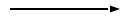
\includegraphics{images/4/scg2sc/arc_main} & \verb+SC_ARC|SC_CONST|SC_POS+
    , \verb+SC_A_CONST|SC_POS+ \\
    
    \hline
	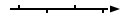
\includegraphics{images/4/scg2sc/pair_const_perm_fuz} & \verb+SC_ARC|SC_CONST|SC_FUZ+
    , \verb+SC_A_CONST|SC_FUZ+ \\
    
    \hline
	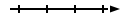
\includegraphics{images/4/scg2sc/pair_const_perm_neg} & \verb+SC_ARC|SC_CONST|SC_NEG+
    , \verb+SC_A_CONST|SC_NEG+ \\
    
    \hline
	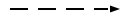
\includegraphics{images/4/scg2sc/pair_var_perm_pos} & \verb+SC_ARC|SC_VAR|SC_POS+
    , \verb+SC_A_VAR|SC_POS+ \\
    
    \hline
	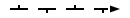
\includegraphics{images/4/scg2sc/pair_var_perm_fuz} & \verb+SC_ARC|SC_VAR|SC_FUZ+
    , \verb+SC_A_VAR|SC_FUZ+ \\
    
    \hline
	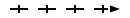
\includegraphics{images/4/scg2sc/pair_var_perm_neg} & \verb+SC_ARC|SC_VAR|SC_NEG+
    , \verb+SC_A_VAR|SC_NEG+ \\
    
    \hline
	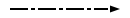
\includegraphics{images/4/scg2sc/pair_meta_perm_pos} & \verb+SC_ARC|SC_METAVAR|SC_POS+
    , \verb+SC_A_METAVAR|SC_POS+ \\
    
    \hline
	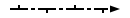
\includegraphics{images/4/scg2sc/pair_meta_perm_fuz} & \verb+SC_ARC|SC_METAVAR|SC_FUZ+
    , \verb+SC_A_METAVAR|SC_FUZ+ \\
    
    \hline
	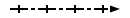
\includegraphics{images/4/scg2sc/pair_meta_perm_neg} & \verb+SC_ARC|SC_METAVAR|SC_NEG+
    , \verb+SC_A_METAVAR|SC_NEG+ \\
    
    \hline
  \end{tabular}
  \label{tab:SCgType2SCType}
\end{table}

Для получения и установки типа sc-элемента используются методы
\lstinline{sc_session::get_type} и
\lstinline{sc_session::change_type}. Более подробную информацию о них
можно найти в doxygen-документации.

Бинарные неориентированные (рис.~\ref{fig:Binary_unorient_pair}) и
ориентированные пары (рис.~\ref{fig:Binary_orient_pair}) в текущей
версии библиотеки libsc нельзя представить в виде атомарных элементов,
а представляются они так, как показано на
рисунках~\ref{fig:Unpack_binary_unorient_pair}~и~\ref{fig:Unpack_binary_orient_pair}
соответственно.

\begin{figure}[h!]
  \centering
  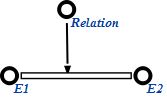
\includegraphics{images/4/scg2sc/Binary_unorient_pair}
  \caption{Бинарная неориентированная пара}
  \label{fig:Binary_unorient_pair}
\end{figure}

\begin{figure}[h!]
  \centering
  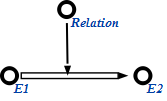
\includegraphics{images/4/scg2sc/Binary_orient_pair}
  \caption{Бинарная ориентированная пара}
  \label{fig:Binary_orient_pair}
\end{figure}

\begin{figure}[h!]
  \centering
  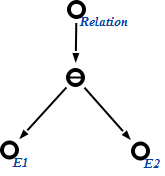
\includegraphics{images/4/scg2sc/Unpack_binary_unorient_pair}
  \caption{Кодирование бинарной неориентированной пары}
  \label{fig:Unpack_binary_unorient_pair}
\end{figure}

\begin{figure}[h!]
  \centering
  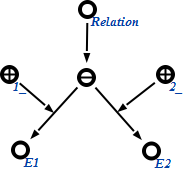
\includegraphics{images/4/scg2sc/Unpack_binary_orient_pair}
  \caption{Кодирование бинарной ориентированной пары}
  \label{fig:Unpack_binary_orient_pair}
\end{figure}

Как видно из приеденных рисунков бинарная неориентированная пара
представляется при помощи трех, а не одного sc-элемента. Бинарная
ориентированная пара представляется при помощи пяти sc-элементов, два
из которых (sc-узлы \idtf{1\_} и \idtf{2\_}) находятся в sc-сегменте
\verb|/proc/keynode| и являются ключевыми узлами.

В следующем разделе мы рассмотрим виды основных обрабатываемых
sc-конструкций.

\subsection{Основные обрабатываемые sc-конструкции}

В sc-памяти sc-элементы могут обрабатываться как поэлементно, так и
целыми группами. Можно выделить два вида таких групп sc-элементов.

Самой распространенной является трехэлементная sc-конструкция. Она
состоит из sc-узла и sc-элемента произвольного типа, которые связаны
sc-дугой. Пример частного случая трехэлементной sc-конструкции
приведен на рис.~\ref{fig:3_sc_constr} (обратите внимание на нумерацию
элементов). Этот частный случай трехэлементной sc-конструкции включает
в качестве первого элемента - константный sc-узел, второго элемента –
константную позитивную sc-дугу, в качестве третьего элемента -
константный sc-узел.

\begin{figure}[h!]
  \centering
  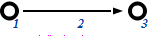
\includegraphics{images/4/3_sc_constr}
  \caption{Трехэлементная sc-конструкция}
  \label{fig:3_sc_constr}
\end{figure}

Не менее распространённой является пятиэлементная sc-конструкция,
частный случай которой приведен на рис.~\ref{fig:5_sc_constr}. Этот
частный случай пятиэлементной sc-конструкции включает в качестве 1-го
элемента – константный sc-узел, 2-го элемента – константную позитивную
sc-дугу, 3-го элемента – константный sc-узел, 4-го элемента -
константную позитивную sc-дугу, 5-го элемент – константный sc-узел.

\begin{figure}[h!]
  \centering
  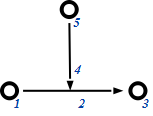
\includegraphics{images/4/5_sc_constr}
  \caption{Пятиэлементная sc-конструкция}
  \label{fig:5_sc_constr}
\end{figure}

Чаще всего пятиэлементная sc-конструкция используется, когда второй
элемент (sc-дуга) уточняется атрибутом, который является пятым
элементом пятиэлементной sc-конструкции.

\subsection{Генерация и удаление sc-конструкций в sc-памяти}

Для генерации одноэлементной sc-конструкции предназначен метод
\lstinline{sc_session::create_el}. Пример генерации константного
sc-узла (если sc-узел будет сгенерирован, то переменная получит в
качестве значения sc-адрес этого узла, иначе она получит в качестве
значения нулевой указатель):

\begin{lstlisting}[texcl]
sc_addr node = session->create_el(
    segment,      // sc-сегмент, в котором будет сгенерирован sc-элемент
    SC_N_CONST // тип sc-элемента
);
\end{lstlisting}

Давайте сгенерируем два константных sc-узла и присвоим им
идентификаторы при помощи метода \lstinline{sc_session::set_idtf} (для
получения идентификатора служит метод
\lstinline{sc_session::get_idtf}):

\begin{lstlisting}[texcl]
sc_addr e1 = session->create_el(segment, SC_N_CONST);
sc_addr e3 = session->create_el(segment, SC_N_CONST);

session->set_idtf(e1, "First");
session->set_idtf(e3, "Third");
\end{lstlisting}

В данной версии модели sc-памяти все sc-элементы всегда имеют
уникальный идентификатор, поэтому не удивляйтесь, если sc-элементы,
для которых вы не устанавливали идентификатор, будут иметь в качестве
него строки странного содержания. Это нормально. Вернемся к нашему
примеру.  Содержимое sc-сегмента segment после выполнение предыдущего
кода показано на рис.~\ref{fig:gen3_f_a_f_before}.

\begin{figure}
  \centering
  
\includegraphics{images/4/gen/gen3_f_a_f_before}
  \caption{Содержимое sc-сегмент segment после генерации двух sc-узлов}
  \label{fig:gen3_f_a_f_before}
\end{figure}

В классе \lstinline{sc_session} есть специальный метод
\lstinline{gen3_f_a_f}, который генерирует второй элемент
трехэлементной sc-конструкции, если известны ее первый и третий
элементы. Его сигнатура выглядит следующим образом:
\begin{lstlisting}[texcl]
class sc_session
{
public:
    // $\dots$
    virtual sc_retval gen3_f_a_f(
        // sc-адрес 1-го элемент
        sc_addr e1,

        // по этому адресу поместить sc-адрес 2-го элемент
        sc_addr *e2,

        // sc-сегмент, в котором будет сгенерирован 2-ой элемент
        sc_segment *seg2,

        // тип 2-го элемента
        sc_type t2,

        // sc-адрес 3-го элемент
        sc_addr e3
    ) = 0;
    // $\dots$
};
\end{lstlisting}

Генерацию трехэлементной sc-конструкции с sc-узлами First и Third
можно провести следующим образом:
\begin{lstlisting}[texcl]
// переменная для sc-адреса 2-го элемента трехэлементной sc-конструкции.
sc_addr e2 = 0;

// Генерация sc-дуги между 1-ым и 3-им элементами.
session->gen3_f_a_f(
    // 1-ый элемент
    e1,

    // в e2 будет помещен sc-адрес 2-го элемента
    &e2,

    // sc-сегмент, в котором будет сгенерирован 2-ой элемент
    segment,

    // тип 2-ого элемента - константная позитивная sc-дуга
    SC_A_CONST|SC_POS,

    // 3-ий элемент
    e3
);
\end{lstlisting}

После выполнения приведенного выше кода содержимое sc-сегмента
\lstinline|segment| изменится так, как показано на
рис.~\ref{fig:gen3_f_a_f_after}.

\begin{figure}[h!]
  \centering
  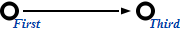
\includegraphics{images/4/gen/gen3_f_a_f_after}
  \caption{Пример генерации трехэлементной sc-конструкции}
  \label{fig:gen3_f_a_f_after}
\end{figure}

Но в некоторых случаях нам не надо получать sc-адрес второго элемента
при использовании метода \lstinline|sc_session::gen3_f_a_f|. В этом
случае можно в качестве второго аргумента этого метода передавать
нулевой указатель:

\begin{lstlisting}[texcl]
// Генерация sc-дуги между 1-ым и 3-им элементами.
session->gen3_f_a_f(
    // 1-ый элемент
    e1,

    // использован нулевой указатель,
    // а это значит что метод не будет возвращать sc-адрес
    // 2-го элемента трехэлементной sc-конструкции
    0,

    // sc-сегмент, в котором будет сгенерирован 2-ой элемент
    segment,

    // тип 2-ого элемента - константная позитивная sc-дуга
    SC_A_CONST|SC_POS,

    // 3-ий элемент
    e3
);
\end{lstlisting}

Запомните этот прием передачи нулевого указателя, потому что он
используется во многих методах и функциях libsc, которые должны
возвращать более одного аргумента.

Теперь обратим внимание на возвращаемое значение метода
\lstinline|sc_session::gen3_f_a_f|. Оно имеет тип
\lstinline|sc_retval| (sc-код возврата) и является просто числом, по
которому можно определить код произошедшей ошибки. Тип
\lstinline|sc_retval| используется во многих методах и функция
библиотеки, и вам необходимо знать о следующих значения этого типа:


\begin{itemize}
\item Константа \lstinline|RV_OK| : функция или метод отработал
  успешно;
\item Константа \lstinline|RV_ERR_GEN| : в процессе работы функции или метода
  произошла ошибка;
\item Константа \lstinline|RV_THEN| : функция или метод сообщает о
  том, что необходим переход по then-ветке условного оператора;
\item Константа \lstinline|RV_ELSE_GEN| : функция или метод сообщает о
  том, что необходим переход по else-ветке условного оператора.
\end{itemize}

В случае успешного выполнения метод \lstinline|sc_session::gen3_f_a_f|
возвратит \lstinline|RV_OK|, а в случае неуспешного –
\lstinline|RV_ERR_GEN|. Проверки можно организовать следующим образом:
\begin{lstlisting}[texcl]
if (session->gen3_f_a_f(...) == RV_OK) {
    // Генерация прошла успешно
} else {
    // Возникла ошибка в процессе генерации
}

// Зная о том, что константа RV\_OK равна 0 можно
// организовать проверку следующим образом.
if (!session->gen3_f_a_f(...)) {
    // Генерация прошла успешно
} else {
    // Возникла ошибка в процессе генерации
}

// Зная о том, что код ошибки неравен 0 можно
// организовать проверку ошибочной ситуации следующим образом.
if (session->gen3_f_a_f(...)) {
    // Возникла ошибка в процессе генерации
}
\end{lstlisting}

Если вы не пишете какой-то специальный устойчивый код, то такие
проверки в алгоритме генерации делать нет необходимости, потому что
ошибочный код возврата метод \lstinline|sc_session::gen3_f_a_f|
возвращает в следующих случаях:
\begin{itemize}
\item не удалось выделить память под генерируемые элементы;
\item sc-сегмент, в котором происходит генерация 2-го элемент
  трехэлементной sc-конструкции закрыт в рамках данной sc-сессии или
  не существует;
\item указан неверный тип 2-го элемента трехэлементной sc-конструкции
  (2-ой элемент должен быть всегда sc-дугой);
\item sc-адреса первого и третьего sc-элементов недействительны в
  рамках данной sc-сессии (эти sc-элементы могут быть уже удалены или
  их sc-сегменты закрыты в рамках данной sc-сессии).
\end{itemize}

Напоследок давайте попробуем написать функцию
\lstinline|my_gen3_f_a_f|, которая делает то же самое, что и метод
\lstinline|sc_session::gen3_f_a_f|. Код этой функции выглядит
следующим образом:
\begin{lstlisting}[texcl]
sc_retval my_gen3_f_a_f(
    sc_session *s, // sc-сессия, через которую будет идти работа
    sc_addr e1,
    sc_addr *e2,
    sc_segment *s2,
    sc_type t2,
    sc_addr e3)
{
    // Генерация 2-го элемента
    sc_addr ce2 = s->create_el(s2, t2);
    if (!ce2)
        return RV_ERR_GEN;

    // Установка начала и конца для sc-дуги ce2
    // (2-го элемента трехэлементной sc-конструкции)
    if (s->set_beg(ce2, e1) || s->set_end(ce2, e3)) {
        // Произошла ошибка и необходимо удалить ce2
        s->erase_el(ce2);
        return RV_ERR_GEN;
    }

    if (e2)
        *e2 = ce2;

    return RV_OK;
}
\end{lstlisting}

В приведенном выше коде для вас должны быть незнакомы только методы
\lstinline|sc_session::set_beg| и \lstinline|sc_session::set_end|. Они
используются для установки начала и конца sc-дуги (для получения
начала и конца используются методы \lstinline|sc_session::get_beg| и
\lstinline|sc_session::get_end| соответственно) и объявлены следующим
образом:
\begin{lstlisting}[texcl]
class sc_session
{
public:
     // $\dots$
     virtual sc_retval set_beg(sc_addr arc, sc_addr beg) = 0;
     virtual sc_retval set_end(sc_addr arc, sc_addr end) = 0;
     // $\dots$
};
\end{lstlisting}

А теперь давайте вернем sc-сегмент \lstinline|segment| из теперешнего
состояния (рис.~\ref{fig:gen3_f_a_f_after}) в состояние, которое
показано на рис.~\ref{fig:gen3_f_a_f_before}. Для этого нам надо
удалить недавно сгенерированную константную позитивную
sc-дугу. Удаление sc-элементов обеспечивается при помощи метода
\lstinline|sc_session::erase_el|:

\begin{lstlisting}[texcl]
class sc_session
{
public:
    // $\dots$
    virtual sc_retval erase_el(sc_addr el) = 0;
    // $\dots$
};
\end{lstlisting}

Следующий код осуществит удаление sc-дуги:

\begin{lstlisting}[texcl]
session->erase_el(e2);
\end{lstlisting}

Теперь добавим еще один константный sc-узел к уже существующим двум:

\begin{lstlisting}[texcl]
sc_addr e5 = session->create_el(segment, SC_N_CONST);
session->set_idtf(e5, "Fifth");
\end{lstlisting}

После выполнения приведенного выше куска кода состояние sc-сегмента
будет таким, как показано на рис.~\ref{fig:gen5_f_a_f_a_f_before}.

\begin{figure}[h!]
  \centering
  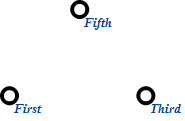
\includegraphics{images/4/gen/gen5_f_a_f_a_f_before}
  \caption{Содержимое sc-сегмента segment после генерации третьего sc-узла ла}
  \label{fig:gen5_f_a_f_a_f_before}
\end{figure}

В классе \lstinline|sc_session| есть специальный метод
\lstinline|gen5_f_a_f_a_f|, который генерирует второй и четвертый
элементы пятиэлементной sc-конструкции, если известны ее первый,
третий и пятый элементы. Его сигнатура выглядит следующим образом:

\begin{lstlisting}[texcl]
class sc_session
{
public:
    // $\dots$
    virtual sc_retval gen5_f_a_f_a_f(
        // sc-адрес 1-го элемент
        sc_addr e1,

        // по этому адресу поместить sc-адрес 2-го элемент
        sc_addr *e2,

        // sc-сегмент, в котором будет сгенерирован 2-ой элемент
        sc_segment *seg2, 

        // тип 2-го элемента
        sc_type t2,

        // sc-адрес 3-го элемент
        sc_addr e3,

        // по этому адресу поместить sc-адрес 4-го элемент
        sc_addr *e2,

        // sc-сегмент, в котором будет сгенерирован 4-ой элемент
        sc_segment *seg4,

        // тип 4-го элемента
        sc_type t4,

        // sc-адрес 5-го элемент
        sc_addr e5
    ) = 0;
    // $\dots$
};
\end{lstlisting}

Генерацию пятиэлементной sc-конструкции с sc-узлами \vidtf{First},
\vidtf{Third}, \vidtf{Fifth} можно провести следующим образом:

\begin{lstlisting}[texcl]
// переменная для sc-адреса 2-го элемента пятиэлементной sc-конструкции.
sc_addr e2 = 0;

// переменная для sc-адреса 4-го элемента пятиэлементной sc-конструкции.
sc_addr e4 = 0;

// Генерация sc-дуги между 1-ым и 3-им, 5-ым и 2-ым элементами.
session->gen5_f_a_f_a_f(
    // 1-ый элемент
    e1,

    // в e2 будет помещен sc-адрес 2-го элемента
    &e2,

    // sc-сегмент, в котором будет сгенерирован 2-ой элемент
    segment,

    // тип 2-ого элемента - константная позитивная sc-дуга
    SC_A_CONST|SC_POS,

    // 3-ий элемент
    e3,

    // в e4 будет помещен sc-адрес 4-го элемента
    &e4,

    // sc-сегмент, в котором будет сгенерирован 4-ой элемент
    segment,

    // тип 4-ого элемента - константная позитивная sc-дуга
    SC_A_CONST|SC_POS,

    // 5-ий элемент
    e5
);
\end{lstlisting}

После выполнения приведенного выше куска кода состояние sc-сегмента
будет таким, как показано на рис.~\ref{fig:gen5_f_a_f_a_f_after}.

Метод \lstinline|sc_session::gen5_f_a_f_a_f| работает аналогично
методу \lstinline|sc_session::gen3_f_a_f|, поэтому для него
справедливо все сказанное ранее про
\lstinline|sc_session::gen3_f_a_f|.

\begin{figure}
  \centering
  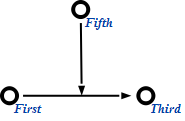
\includegraphics{images/4/gen/gen5_f_a_f_a_f_after}
  \caption{Пример генерации пятиэлементной sc-конструкции}
  \label{fig:gen5_f_a_f_a_f_after}
\end{figure}

%%% Local Variables: 
%%% mode: latex
%%% TeX-master: "main"
%%% End: 
